\section{实验}

本节详细介绍了用于评估 PhyPrompt 在物理驱动视频生成任务上的有效性的实验方法。我们的评估侧重于三个主要方面：(1) 生成的视频的物理合理性和语义保真度，(2) 学习的 PhyPrompt 重写器在不同文本到视频 (T2V) 生成器之间的可迁移性，以及 (3) 消融研究，调查我们提出的方法中关键组件的贡献。
\\
\textbf{文本到视频生成器。}
PhyPrompt 的性能使用多种当前最先进的 T2V 扩散模型进行评估，参数数量范围从 8.6 亿到 50 亿：

\begin{itemize}
\item \textbf{Lavie}~\cite{wang2023lavie}：一个 860M 参数模型，利用级联潜在扩散，在 Vimeo25M 数据集上进行训练。它能够生成长度长达 8 秒、分辨率为 1280×720 像素的视频。
\item \textbf{VideoCrafter2}~\cite{chen2024videocrafter2}：此 1.2B 参数模型采用基于扩散的架构。它使用低质量视频和高质量图像的组合进行训练，以提高运动一致性和视觉保真度，以 512×512 分辨率生成持续时间长达 8 秒的视频。
\item \textbf{CogVideoX-2B}~\cite{yang2024cogvideox}：2B 参数模型，具有 3D 变分自动编码器和具有自适应 LayerNorm 的专家 Transformer。它可以生成长达 6 秒、分辨率为 720×480 的视频。
\item \textbf{CogVideoX-5B}~\cite{yang2024cogvideox}：这个 5B 参数模型共享 CogVideoX-2B 的架构，但受益于更大规模的训练数据。它可生成长度长达 6 秒、分辨率为 720×480 的视频。
\end{itemize}
为了确保所有模型的评估一致，生成的视频被标准化为时长 6 秒、帧速率为 4 FPS、分辨率为 720×480 像素。补充材料中提供了 T2V 生成设置的详细配置。
\\
\textbf{提示增强器。}
PhyPrompt 变体是通过使用 1.5B、3B 和 7B 参数微调 Qwen2.5-Instruct 检查点获得的。
为了进行比较，我们包括四个自动提示细化基线：Promptist~\cite{hao2023promptist}, PhyT2V~\cite{xue2024phyt2v}, GPT-4o~\cite{achiam2023gpt-4o}、和 DeepSeek-V3~\cite{liu2024deepseek-v3}.
\\
\textbf{数据集。}
我们的方法在 VideoPhy2 基准上进行评估~\cite{bansal2025videophy2}。该基准包含专门设计用于评估视频生成中的物理常识的各种提示集合，包括与重力、碰撞、流体动力学和其他基本物理现象相关的场景。
\\
\textbf{评估指标。}
按照~\cite{bansal2025videophy2} 的设置，生成视频从两个标准进行评估：语义遵循度（SA）和物理常识（PC）。每个标准均采用 5 点李克特量表，范围从“非常不可能”(1) 到“非常可能”(5)。我们从测试集中随机抽取 500 个提示词，并报告生成视频满足以下条件的百分比：
\begin{itemize}
\item \textbf{语义遵循度（SA $\geq$ 4)}：准确描述提示中描述的预期内容的视频的百分比。
\item \textbf{物理常识（PC $\geq$ 4)}：真实遵循基本物理原理的视频百分比。
\item \textbf{联合表现（SA $\geq$  4、PC $\geq$  4)}：同时获得高分的视频百分比（即 $\geq$ 4）语义遵循度和物理真实性。
\end{itemize}

\subsection{生成视频的质量评估}
\label{sec:quality}
我们衡量每种提示词重写策略在搭配 \textbf{CogVideoX-2B}\cite{yang2024cogvideox} 时，对 \textbf{语义遵循度（SA）} 和 \textbf{物理常识（PC）} 的改善。
表~\ref{tab:quality} 报告了 \textsc{VideoPhy2} 基准~\cite{bansal2025videophy2} 中 500 个提示词上的结果。

\begin{table*}
\centering
\caption{\textbf{CogVideoX-2B 的 VideoPhy2 质量结果。}
对于每个提示重写策略，我们报告视频评分的百分比 $\ge\!4$ 对于语义遵循度（SA）和物理常识（PC），它们的联合百分比（SA \& PC），以及平均 SA/PC 分数（平均 SA、平均 PC）。}
\vspace{0.1in}
\label{tab:quality}
\setlength{\tabcolsep}{3mm}{
\renewcommand\arraystretch{0.9}
\resizebox{\linewidth}{!}{
\begin{tabular}{lccccc}
\toprule
\textbf{Enhanced Model} &
\textbf{SA (\%)} $\uparrow$ &
\textbf{PC (\%)} $\uparrow$ &
\textbf{SA \& PC (\%)} $\uparrow$ &
\textbf{Avg SA} $\uparrow$ &
\textbf{Avg PC} $\uparrow$ \\
\midrule
N/A (Original Prompt)           & 43.4 & 55.8 & 32.2 & 3.842 & 4.410 \\
Promptist~\cite{hao2023promptist}     & 41.2 & 58.2 & 30.2 & 3.782 & 4.452 \\
PhyT2V~\cite{xue2024phyt2v}     & 45.0 & 62.0 & 36.2 & 3.854 & 4.522 \\
\midrule
Qwen2.5-1.5B              & 37.6 & 64.0 & 31.8 & 3.616 & 4.562 \\
PhyPrompt-1.5B            & 42.8 & 65.4 & 37.4 & 3.800 & 4.580 \\
\addlinespace[4pt]
Qwen2.5-3B                & 40.0 & 64.2 & 32.0 & 3.754 & 4.582 \\
PhyPrompt-3B              & 46.4 & 64.8 & 39.6 & 3.868 & 4.556 \\
\addlinespace[4pt]
Qwen2.5-7B                & 44.8 & 64.6 & 34.2 & 3.848 & 4.586 \\
PhyPrompt-7B              & 47.8 & \textbf{66.8} & \textbf{40.8} & 3.878 & \textbf{4.590} \\
\midrule
GPT-4o                    & 47.0 & 60.0 & 37.0 & 3.932 & 4.488 \\
DeepSeek-V3               & \textbf{48.4} & 64.6 & 38.6 & \textbf{3.968} & 4.564 \\
\bottomrule
\end{tabular}%
}}
\end{table*}

\noindent \textbf{PhyPrompt 的有效性。}
Promptist~\cite{hao2023promptist} 将 PC 从 55.8\% 提高到 58.2\%，但 SA 从 43.4\% 降至 41.2\%，使联合得分从 32.2\% 降至 30.2\%。这说明通用文本到图像适配器无法在视频领域可靠地平衡语义与物理。PhyT2V~\cite{xue2024phyt2v} 达到 45.0\% SA 和 62.0\% PC（36.2\% 联合），展示了迭代 LLM 反馈的价值，但需要多轮提示和复杂的后退机制。相比之下，三个 PhyPrompt 检查点在所有指标上都优于原始提示词和现有基线。7B 模型收益最大，达到 47.8\% SA、66.8\% PC 和 40.8\% 联合成功率，相比基线绝对提升 8.6 个百分点，相比 Promptist 提升 10.6 个百分点。值得注意的是，即使 1.5B 版本也达到 37.4\% 联合得分，比 Promptist 高 7.2 个百分点，同时仅使用 GPT-4o 约 1/10 的参数量。所有模型规模上的一致改进验证了两阶段训练方法的有效性：以物理为中心的 SFT 与基于动态奖励的 RL 相结合。

\noindent\textbf{相对于通用大型语言模型的优势。}
PhyPrompt 表明，在物理感知视频生成上，领域专用训练比单纯扩大参数规模更有效。与 GPT-4o~\cite{achiam2023gpt-4o} 相比，PhyPrompt-7B 达到几乎相同的 SA（47.8\% vs. 47.0\%），同时带来更高的 PC（66.8\% vs. 60.0\%）和联合表现（40.8\% vs. 37.0\%）。这 6.8 个百分点的 PC 优势来自三个因素：（i）针对视频质量指标而非文本似然进行端到端 RL 优化~\cite{ouyang2022training}，（ii）以物理为中心的 CoT 预训练编码了领域特定推理~\cite{wei2022chain}，（iii）动态奖励课程平衡了双目标~\cite{bengio2009curriculum}。DeepSeek-V3~\cite{liu2024deepseek-v3} 虽然参数多约 100 倍（671B），但在 PC（64.6\% vs. 66.8\%）和联合表现（38.6\% vs. 40.8\%）上仍落后于 PhyPrompt-7B，说明通用预训练不能替代任务特定反馈~\cite{hoffmann2022training}。PhyPrompt-3B 用不到 GPT-4o 1\% 的参数量即可达到相近水平，也呼应了近期发现：专用小模型可以在聚焦任务上超过通用大模型~\cite{muennighoff2023scaling}。总体而言，我们的结果支持一种新兴观点：带有直接任务反馈的领域目标训练，比单独扩展模型规模更具参数效率~\cite{kaplan2020scaling,wei2022emergent}.


\subsection{跨生成器的零样本迁移}
\label{sec:transfer}
\begin{figure*}[t]
    \centering
   \resizebox{1.0\textwidth}{!}{%
    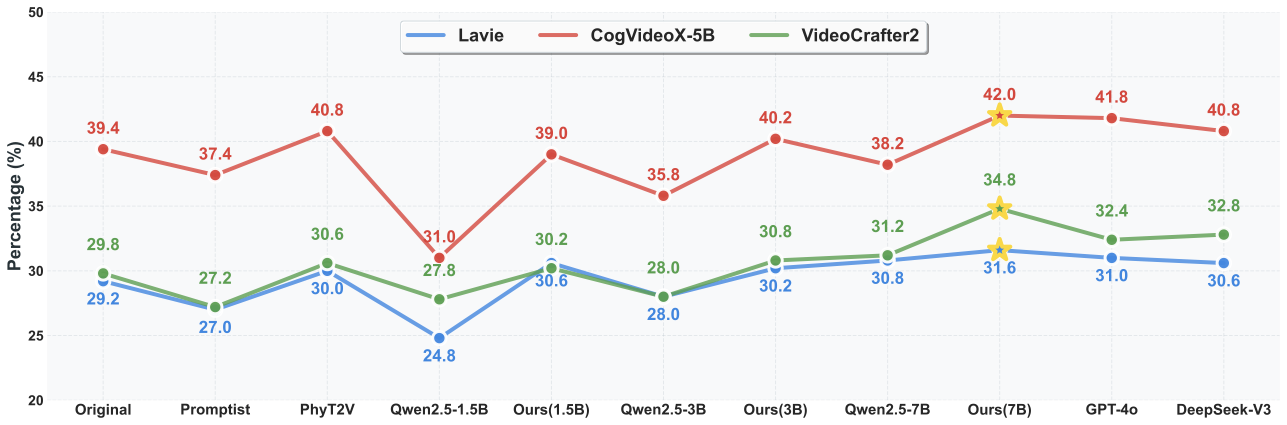
\includegraphics{figures_zh/all_results_combined.png}
    }
    \vspace{-0.15in}
    \caption{\textbf{PhyPrompt 的跨生成器迁移。} 图中比较了不同提示词增强方法在三种文本到视频生成模型（Lavie、CogVideoX-5B 和 VideoCrafter2）上的联合物理常识与语义遵循度（PC \& SA）指标。本文方法在三个视频生成后端上均稳定优于基线方法（Original、Promptist、PhyT2V）和同规模 Qwen2.5 模型。最高性能（42.0\%）由 7B 模型在 CogVideoX-5B 上取得。金色星号表示每个生成器上的最佳方法。}
    \label{fig:transfer}
    \vspace{-0.2in}
\end{figure*}

\begin{figure}[!htbp]
  \centering
    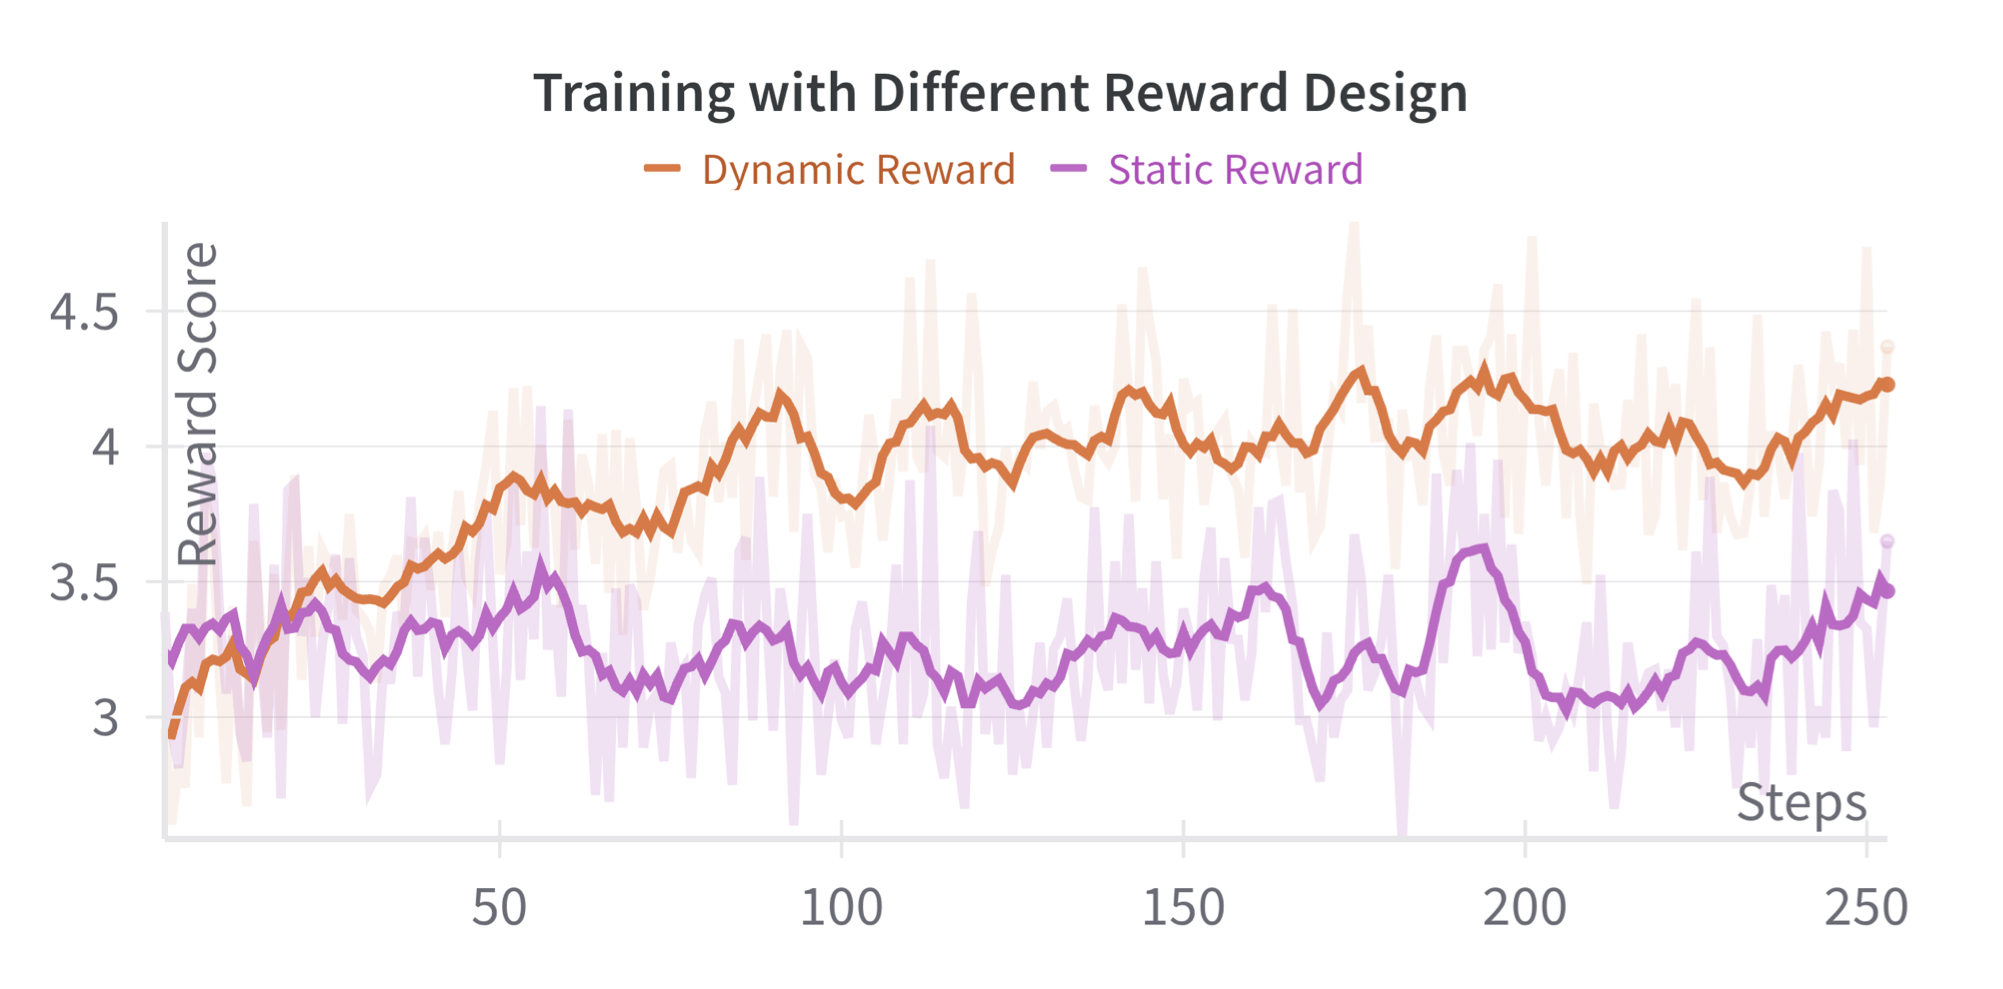
\includegraphics[width=1.0\linewidth]{figures_zh/reward.png}
    \captionof{figure}{动态（橙色）和静态（紫色）奖励公式下的训练奖励曲线。每条线均采用 10 步移动平均线进行平滑处理；浅色阴影痕迹显示未平滑的每集奖励。与静态基线 (3.5) 相比，动态课程收敛速度更快，稳定程度更高 (4.2)，表明优化更有效。}
    \label{fig:reward_curve}
  \vspace{-1em}
\end{figure}

为了验证 PhyPrompt 与生成器无关的迁移，我们在三种架构不同的扩散模型上评估 PhyPrompt-7B（仅在 CogVideoX-2B 上训练）：Lavie (860M)、VideoCrafter2 (1.2B) 和 CogVideoX-5B (5B)。我们为每个生成器的每种方法生成 500 个视频并报告联合 SA\&PC得分~\cref{fig:transfer}。完整的结果出现在补充中。

\noindent\textbf{联合度量改进。} 原始提示达到基线联合分数 29.2\% （Lavie），29.8\% （VideoCrafter2）和 39.4\% （CogVideoX-5B）。 Promptist 将性能降低至 27.0\%, 27.2\%、37.4\%， 分别。 PhyPrompt 大大超过了每个生成器的基线：Lavie 达到 31.6\% (+8.2\% VideoCrafter2 达到 34.8\% (+16.8\% 超过原始值），CogVideoX-5B 达到 42.0\% (+6.6\% 超过原来）。较小的 PhyPrompt 变体（1.5B 和 3B）表现出相同的改进模式，3B 模型达到 30.2\%, 30.8\%、40.2\% 分别确认我们的训练方法可以有效地跨模型大小进行扩展。

\noindent\textbf{与其他重写器的比较。} PhyT2V 比 Promptist 有所改进，但在所有生成器上的表现均低于 PhyPrompt，达到 30.0\%, 30.6\%、40.8\% 分别在 Lavie、VideoCrafter2 和 CogVideoX-5B 上。 GPT-4o、DeepSeek-V3 和大小匹配的 Qwen 基线在联合指标上同样落后于 PhyPrompt。在 VideoCrafter2 上，最佳替代方案（DeepSeek-V3，32.8\%) 仍为 2.0\% 低于 PhyPrompt-7B； Lavie 和 CogVideoX-5B 也有类似的利润。

\noindent\textbf{零样本迁移。} 所有 PhyPrompt 变体均仅在 CogVideoX-2B 输出上进行微调，但无需任何后端调整即可在 Lavie 和 VideoCrafter2 上产生显着增益。这证实了真正的零样本迁移，其中物理感知重写捕获与模型无关的物理先验，而不是利用生成器特定的偏差。语言模型参数高效提示调优的相关工作也同样证明了跨模型泛化能力~\cite{lester2021power,li2021prefix}，并且基于强化学习的提示适配器已被证明可以跨模态迁移~\cite{hao2023promptist}。通过消除任何特定扩散架构的物理约束，PhyPrompt 消除了对每个生成器进行微调的需要，减少了计算开销并实现了跨不同 T2V 管道的快速部署。



\subsection{消融研究}
为了理清 PhyPrompt 增益的来源，我们进行了两次互补的消融。
首先，我们研究 GRPO 微调期间奖励计划的选择如何影响性能。
其次，我们测试两阶段流程（SFT 和 RL）的必要性。
结果表明，课程奖励和两阶段程序都贡献了相当大的、互补的改进。

\subsubsection{奖励设计}
\label{sec:reward_design}

\begin{figure*}[!htbp]
  \centering
  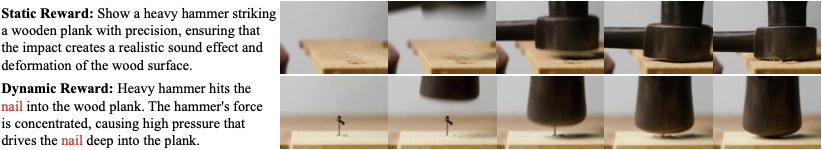
\includegraphics[width=\textwidth]{figures_zh/reward_demo.png}
   \caption{\textbf{“锤子和钉子”场景下 CogVideoX-2B 输出的逐帧比较。}
上排显示静态奖励提示词的结果
“\textit{展示重锤精确敲击木板，确保撞击产生逼真的声音效果和木材表面的变形。}”
锤子撞击木板，但画面中看不到钉子，也没有钉子被钉入。
下排显示动态奖励提示词的结果
“\textit{用重锤将钉子敲入木板上。锤子的力量集中，产生高压，将钉子深深地钉入木板。}”
此处，钉子出现在第 1 帧中，穿过第 2-3 帧逐渐压入木材中，并在第 4 帧中实现完全穿透，具有真实的木材变形和进入深度。}
\vspace{-1em}
  \label{fig:hammer_frames}
\end{figure*}

为了证明语义遵循度（SA）和物理常识（PC）本质上是相互冲突的目标，我们进行了系统的消融，比较了四种奖励策略：（i）~仅 SA 优化（$w_{\text{sa}} = 1.0, w_{\text{pc}} = 0.0$), (ii)~仅限 PC 优化 ($w_{\text{sa}} = 0.0, w_{\text{pc}} = 1.0$), (iii)~静态平衡权重 ($w_{\text{sa}} = w_{\text{pc}} = 0.5$），以及（iv）~我们的动态课程（方程式~\ref{eq:total_reward}）。我们使用 Qwen2.5-7B-Instruct 作为基础模型，使用 CogVideoX-2B 作为视频生成器。结果显示在 \cref{fig:reward_curve} 还有~\cref{tab:reward_ablation}.

\noindent\textbf{目标之间的负迁移。}
\cref{tab:reward_ablation} 揭示了严重的负迁移。仅 SA 训练将语义遵循度提高到 45.6\% (+2.2\% 超过基线），但物理常识下降至 52.8\% ($-3.0\%$），产生更差的联合表现（31.6\% 对比 32.2\% 基线）。相反，仅使用 PC 的培训达到 65.2\% 物理成绩（+9.4\%）但将语义遵循度降低到 39.4\% ($-4.0\%$），只有边际联合改进（33.4\%）。这种对立关系表明 SA 和 PC 无法通过朴素的单目标优化来共同最大化。静态平衡加权达到35.4\% 联合成功率，优于任一极端，但仍为 5.4\% 下面是我们的动态课程。

\noindent\textbf{动态课程超出了单一目标的上界。}
我们的动态课程达到 SA = 47.8\% 且 PC = 66.8\%。值得注意的是，这在语义遵循度方面优于仅 SA 训练（47.8\% 对比 45.6\%），同时在物理常识方面优于仅使用 PC 的训练（66.8\% 对比 65.2\%）。换句话说，我们的方法在其目标上击败了每位专家。这表明将两个目标与课程一起优化比单独优化其中一个目标会产生更好的结果~\cite{caruana1997multitask,yu2020gradient,standley2020tasks}。


我们假设语义描述建立了物体身份和关系（例如“球”和“倾斜”），而物理约束通过动力学来完善这些身份和关系（例如“加速”和“在重力作用下”）。高质量的物理描述需要精准的语义基础~\cite{scholkopf2021toward}：如果不首先确定存在什么物体，就无法指定现实的力。仅 SA 优化发现具有良好语义结构的提示，但缺乏物理约束的细化压力。仅适用于 PC 的优化会生成物理上详细的提示，但缺乏语义连贯性来有效组织这些细节。我们的课程利用了这两个信号：SA 建立组合支架，然后 PC 通过物理特异性细化这个结构，起到隐式正则化的作用~\cite{liebel2018auxiliary}。这种分阶段的方法发现了单目标轨迹无法到达的区域中的提示~\cite{bengio2009curriculum}，解释我们如何超过两个上界。

与静态平衡权重相比，我们的动态课程在所有三个 VideoPhy2 指标上都有所改进，这表明依赖时间的时间表可以增强两个目标，而不是权衡一个目标。值得注意的是，该课程实现了比仅 SA 培训更高的 SA（47.8\% 对比 45.6\%），表明分阶段方法可以更有效地探索提示空间。

\noindent\textbf{案例研究：锤子和钉子。}
\cref{fig:hammer_frames} 说明了质量影响。对于提示“\textit{用重锤将钉子敲入木板}，”静态平衡权重生成的视频中，锤子撞击木板，但钉子不存在（语义失败）。相比之下，我们的动态课程会生成明确命名钉子并描述力动态的提示，从而产生物理连贯的序列，其中钉子逐渐被钉入木头并产生真实的变形。这例证了我们的课程如何避免纯 PC 优化中固有的语义漂移，同时捕获纯 SA 训练错过的物理细节。



\begin{table}[t]
  \centering
  \caption{\textsc{VideoPhy2} 上的奖励权重消融。
           固定权重策略表现出 SA-PC 权衡；
           我们的动态课程（\cref{eq:weights}）达到帕累托优势。}
  \label{tab:reward_ablation}
  \vspace{0.05in}
  \small
  \begin{tabular}{lccc}
    \toprule
    \textbf{奖励函数} & \textbf{SA（\%)} & \textbf{PC（\%)} & \textbf{联合（\%)} \\
    \midrule
    没有训练（基线）     & 43.4 & 55.8 & 32.2 \\
    \midrule
    SA分数              & 45.6 & 52.8 & 31.6 \\
    PC分数              & 39.4 & 65.2 & 33.4 \\
    静态         & 45.0 & 60.2 & 35.4 \\
    \midrule
    \textbf{动态（本文）}    & \textbf{47.8} & \textbf{66.8} & \textbf{40.8} \\
    \bottomrule
  \end{tabular}
\end{table}
